% Chapter 1
%\chapter{مقدمه}

\section{بررسی نتایج}

\subsection{
	مجموعه داده
	\lr{\texttt{\fontspec{Times New Roman} MNIST}}%
	\LTRfootnote{Modified National Institute of Standards and Technology}
}
اکنون نتایج مربوط به مجموعه داده
\lr{MNIST}
بررسی خواهد شد که شکل
\ref{result_mnist_mlp}
نتایج مقایسه روش
\lr{SimFedSwap}
با سایر روش‌های مرجع را با استفاده از مدل
\lr{MLP}
به تصویر می‌کشد.
\begin{figure}[t]
	\centering
	\subfigure[
	دید کلی از نتیجه
	\qquad\hspace{3mm}]{
		\label{result_mnist_mlp_mid}
		\includegraphics*[width=.441\textwidth]{images/chap5/result/mnist/acc_mid_mlp.png}
	}
	\hspace{0.8mm}
	\subfigure[
	بزرگ‌نمایی شده بخش اصلی					
	\qquad\hspace{5mm}]{
		\label{result_mnist_mlp_zoom}
		\includegraphics*[width=.441\textwidth]{images/chap5/result/mnist/acc_zoom_mlp.png}
	}
	\caption{
		مقایسه منحنی‌های دقت در مجموعه داده
		\lr{MNIST}
		با استفاده از مدل
		\lr{MLP}.
	}
	\label{result_mnist_mlp}
\end{figure}
همچنین، پارامترهای به‌کاررفته در این اجرا در جدول
\ref{tabel_parameter_mnist} 
به نمایش درآمده‌اند.
%\addtolength{\tabcolsep}{-0.5mm}
\begin{table}[t]
	\centering
	\caption{
		پارامترهای اجرا در مجموعه داده
		\lr{MNIST}
	}
	\label{tabel_parameter_mnist}
	%	\scalebox{0.985}{
		\begin{tabular}{ccccccccccccc}
			\hline
			\specialcell{مجموعه\\داده} &
			\specialcell{نحوه\\جابه‌جایی} &
			\specialcell{توزیع\\داده} &
			$K$ &
			$B$ &
			$C$ &
			$SP$ &
			$\eta$ &
			$E$ &
			$h_1$ &
			$h_2$
			\\
			\hline
			\lr{MNIST} &
			\lr{MSS} &
			نرمال &
			\lr{10} &
			\lr{32} &
			\lr{1.0} &
			\lr{1.0} &
			\lr{0.001} &
			\lr{1} &
			\lr{5} &
			\lr{3}
			\\
		\end{tabular}
		%	}
\end{table}
نکته قابل توجه این است که منحنی‌های
\lr{FedAvg} 
و
\lr{FedSwap} 
به عنوان منحنی‌های نهایی و مرجع بر روی سایر منحنی‌ها قرار گرفته‌اند. در صورتی که رنگ متفاوتی در نمودار دیده شود، این موضوع نشان‌دهنده اختلاف عملکرد روش مربوطه در آن نقطه خواهد بود. این تغییر ممکن است نشان‌دهنده عملکرد بهتر یا ضعیف‌تر در مقایسه با دیگر روش‌ها باشد و می‌تواند به عنوان مبنایی برای مقایسه و تحلیل مورد توجه قرار گیرد.




همان‌طور که در شکل
\ref{result_mnist_mlp} 
مشاهده می‌شود، روش‌های مبتنی‌بر جابه‌جایی به شکل بسیار ناچیزی از روش
\lr{FedAvg} 
نتایج مطلوب‌تری را ارائه داده‌اند. نکته قابل توجه این است که همه روش‌های مبتنی‌بر جابه‌جایی عملکردی مشابه داشته‌اند. برای بررسی دقیق‌تر این اجرا، منحنی‌های خطا در شکل
\ref{app_result_mnist_mlp}
پیوست، قابل مشاهده هستند.


در شکل
\ref{result_mnist_cnn}
همان آزمایش قبلی تکرار شده، با این تفاوت که این مرتبه از مدل شبکه عصبی
\lr{CNN}
استفاده شده است. همان‌طور که دیده می‌شود، تقریباً تمامی روش‌ها عملکرد مشابهی داشته‌اند. این نکته نشان می‌دهد که وقتی شبکه به راحتی به دقت بالایی می‌رسد، تفاوتی در نتایج بین روش‌ها دیده نمی‌شود. برای جزئیات بیشتر این اجرا، منحنی‌های خطا در شکل
\ref{app_result_mnist_cnn}
پیوست، آمده‌اند.


\begin{figure}[t]
	\centering
	\subfigure[
	دید کلی از نتیجه
	\qquad\hspace{3mm}]{
		\label{result_mnist_cnn_mid}
		\includegraphics*[width=.48\textwidth]{images/chap5/result/mnist/acc_mid_cnn.png}
	}
	\hspace{0.8mm}
	\subfigure[
	بزرگ‌نمایی شده بخش اصلی					
	\qquad\hspace{5mm}]{
		\label{result_mnist_cnn_zoom}
		\includegraphics*[width=.48\textwidth]{images/chap5/result/mnist/acc_zoom_cnn.png}
	}
	\caption{
		مقایسه منحنی‌های دقت در مجموعه داده
		\lr{MNIST}
		با استفاده از مدل
		\lr{CNN}.
	}
	\label{result_mnist_cnn}
\end{figure}





\FloatBarrier
\subsection{
	مجموعه داده
	\lr{\texttt{\fontspec{Times New Roman} CIFAR-10}}%
	\LTRfootnote{Canadian Institute For Advanced Research}
}
اکنون نتایج مربوط به مجموعه داده
\lr{CIFAR-10}
بررسی خواهد شد که شکل
\ref{result_cifar10_equal}
نتایج مقایسه روش
\lr{SimFedSwap}
با سایر روش‌های مرجع را با توزیع داده یکنواخت بین کاربران به تصویر می‌کشد.
پارامترهای استفاده شده در این آزمایش نیز در جدول
\ref{tabel_parameter_cifar10}
به نمایش درآمده‌اند.


\begin{figure}[t]
	\centering
	\subfigure[
	دید کلی از نتیجه
	\qquad\hspace{3mm}]{
		\label{result_cifar10_equal_mid}
		\includegraphics*[width=.48\textwidth]{images/chap5/result/cifar10/acc_mid_equal.png}
	}
	\hspace{0.8mm}
	\subfigure[
	بزرگ‌نمایی شده بخش اصلی					
	\qquad\hspace{5mm}]{
		\label{result_cifar10_equal_zoom}
		\includegraphics*[width=.48\textwidth]{images/chap5/result/cifar10/acc_zoom_equal.png}
	}
	\caption{
		مقایسه منحنی‌های دقت در مجموعه داده
		\lr{CIFAR-10}
		با توزیع داده یکنواخت.
	}
	\label{result_cifar10_equal}
\end{figure}


%\addtolength{\tabcolsep}{-0.5mm}
\begin{table}[t]
	\centering
	\caption{
		پارامترهای اجرا در مجموعه داده
		\lr{CIFAR-10}
	}
	\label{tabel_parameter_cifar10}
	%	\scalebox{0.985}{
		\begin{tabular}{ccccccccccccc}
			\hline
			\specialcell{مجموعه\\داده} &
			\specialcell{شبکه\\عصبی} &
			\specialcell{نحوه\\جابه‌جایی} &
			$K$ &
			$B$ &
			$C$ &
			$SP$ &
			$\eta$ &
			$E$ &
			$h_1$ &
			$h_2$
			\\
			\hline
			\lr{CIFAR-10} &
			\lr{Conv} &
			\lr{MSS} &
			\lr{10} &
			\lr{64} &
			\lr{1.0} &
			\lr{1.0} &
			\lr{0.001} &
			\lr{2} &
			\lr{3} &
			\lr{10}
			\\
		\end{tabular}
		%	}
\end{table}


همان‌طور که در شکل
\ref{result_cifar10_equal}
مشاهده می‌شود، روش‌های مبتنی‌بر جابه‌جایی نسبت به روش
\lr{FedAvg}
عملکرد متمایزی داشته‌اند. با این حال، این روش‌ها در یک سطح عملکردی نزدیک به هم قرار گرفته‌اند. به‌طور کلی، با وجود اختلافات جزئی، روش‌های مبتنی‌بر شباهت در مقایسه با روش
\lr{FedSwap}
کمی بهتر عمل کرده‌اند. برای آگاهی از جزئیات بیشتر، به منحنی‌های خطا در شکل
\ref{app_result_cifar10_equal}
پیوست، توجه نمایید.


در شکل
\ref{result_cifar10_normal}%
، آزمایش قبلی دوباره اجرا شده، اما این بار از توزیع داده نرمال استفاده شده است. مشاهده می‌شود که در این وضعیت نیز روش‌های مبتنی‌بر جابه‌جایی، عملکرد بهتری نسبت به روش
\lr{FedAvg}
داشته‌اند. البته، نتایج حاصل از روش‌های جابه‌جایی تقریباً مشابه بوده و تفاوت قابل توجهی بین آن‌ها دیده نمی‌شود. برای مشاهده جزئیات بیشتر، می‌توان به منحنی‌های خطا در شکل
\ref{app_result_cifar10_normal}
پیوست، مراجعه کرد.

\begin{figure}[t]
	\centering
	\subfigure[
	دید کلی از نتیجه
	\qquad\hspace{3mm}]{
		\label{result_cifar10_normal_base}
		\includegraphics*[width=.48\textwidth]{images/chap5/result/cifar10/acc_base_normal.png}
	}
	\hspace{0.8mm}
	\subfigure[
	بزرگ‌نمایی شده بخش اصلی					
	\qquad\hspace{5mm}]{
		\label{result_cifar10_normal_zoom}
		\includegraphics*[width=.48\textwidth]{images/chap5/result/cifar10/acc_zoom_normal.png}
	}
	\caption{
		مقایسه منحنی‌های دقت در مجموعه داده
		\lr{CIFAR-10}
		با توزیع داده نرمال.
	}
	\label{result_cifar10_normal}
\end{figure}




\FloatBarrier
\subsection{
	مجموعه داده
	\lr{\texttt{\fontspec{Times New Roman} CINIC-10}}%
	\LTRfootnote{CIFAR-10 and ImageNet Combined}
}

اکنون نتایج مربوط به مجموعه داده
\lr{CINIC-10}
بررسی خواهد شد که شکل
\ref{result_cinic10}
نتایج مقایسه روش
\lr{SimFedSwap}
با سایر روش‌های مرجع را به تصویر می‌کشد.
همچنین، پارامترهای به کار رفته در این آزمایش در جدول
\ref{tabel_parameter_cinic10}
ارائه شده‌اند.

\begin{figure}[t]
	\centering
	\subfigure[
	دید کلی از نتیجه
	\qquad\hspace{3mm}]{
		\label{result_cinic10_mid}
		\includegraphics*[width=.48\textwidth]{images/chap5/result/cinic10/acc_mid.png}
	}
	\hspace{0.8mm}
	\subfigure[
	بزرگ‌نمایی شده بخش اصلی					
	\qquad\hspace{5mm}]{
		\label{result_cinic10_zoom}
		\includegraphics*[width=.48\textwidth]{images/chap5/result/cinic10/acc_zoom.png}
	}
	\caption{
		مقایسه منحنی‌های دقت در مجموعه داده
		\lr{CINIC-10}.
	}
	\label{result_cinic10}
\end{figure}


%\addtolength{\tabcolsep}{-0.5mm}
\begin{table}[t]
	\centering
	\caption{
		پارامترهای اجرا در مجموعه داده
		\lr{CINIC-10}
	}
	\label{tabel_parameter_cinic10}
	%	\scalebox{0.985}{
		\begin{tabular}{ccccccccccccc}
			\hline
			\specialcell{مجموعه\\داده} &
			\specialcell{شبکه\\عصبی} &
			\specialcell{نحوه\\جابه‌جایی} &
			\specialcell{توزیع\\داده} &
			$K$ &
			$B$ &
			$C$ &
			$SP$ &
			$\eta$ &
			$E$ &
			$h_1$ &
			$h_2$
			\\
			\hline
			\lr{CINIC-10} &
			\lr{Conv} &
			\lr{MSS} &
			نرمال &
			\lr{30} &
			\lr{64} &
			\lr{0.5} &
			\lr{1.0} &
			\lr{0.001} &
			\lr{1} &
			\lr{2} &
			\lr{5}
			\\
		\end{tabular}
		%	}
\end{table}


در شکل
\ref{result_cinic10}
به‌وضوح می‌توان مشاهده کرد که روش‌های مبتنی‌بر جابه‌جایی در مقایسه با روش
\lr{FedAvg}%
، عملکرد متفاوتی داشته‌اند. هرچند، این روش‌ها همچنان در یک سطح عملکردی نزدیک به هم قرار دارند و تفاوت‌های عمده‌ای میان آن‌ها دیده نمی‌شود. برای بررسی دقیق‌تر، منحنی‌های خطا در شکل
\ref{app_result_cinic10}
پیوست، به تفصیل آمده‌اند.







\FloatBarrier
\subsection{
	مجموعه داده
	\lr{\texttt{\fontspec{Times New Roman} FEMNIST}}%
	\LTRfootnote{Federated Extended MNIST}
}
در این مجموعه داده، تعداد داده‌ها در هر کلاس یکسان نیست و کلاس‌های مختلف دارای تعداد متفاوتی از داده‌ها هستند. شکل
\ref{count_all_classes}%
، تعداد داده‌های هر کلاس و نحوه نام‌گذاری آن‌ها را نشان می‌دهد.


\begin{figure}[t]
	\centering
	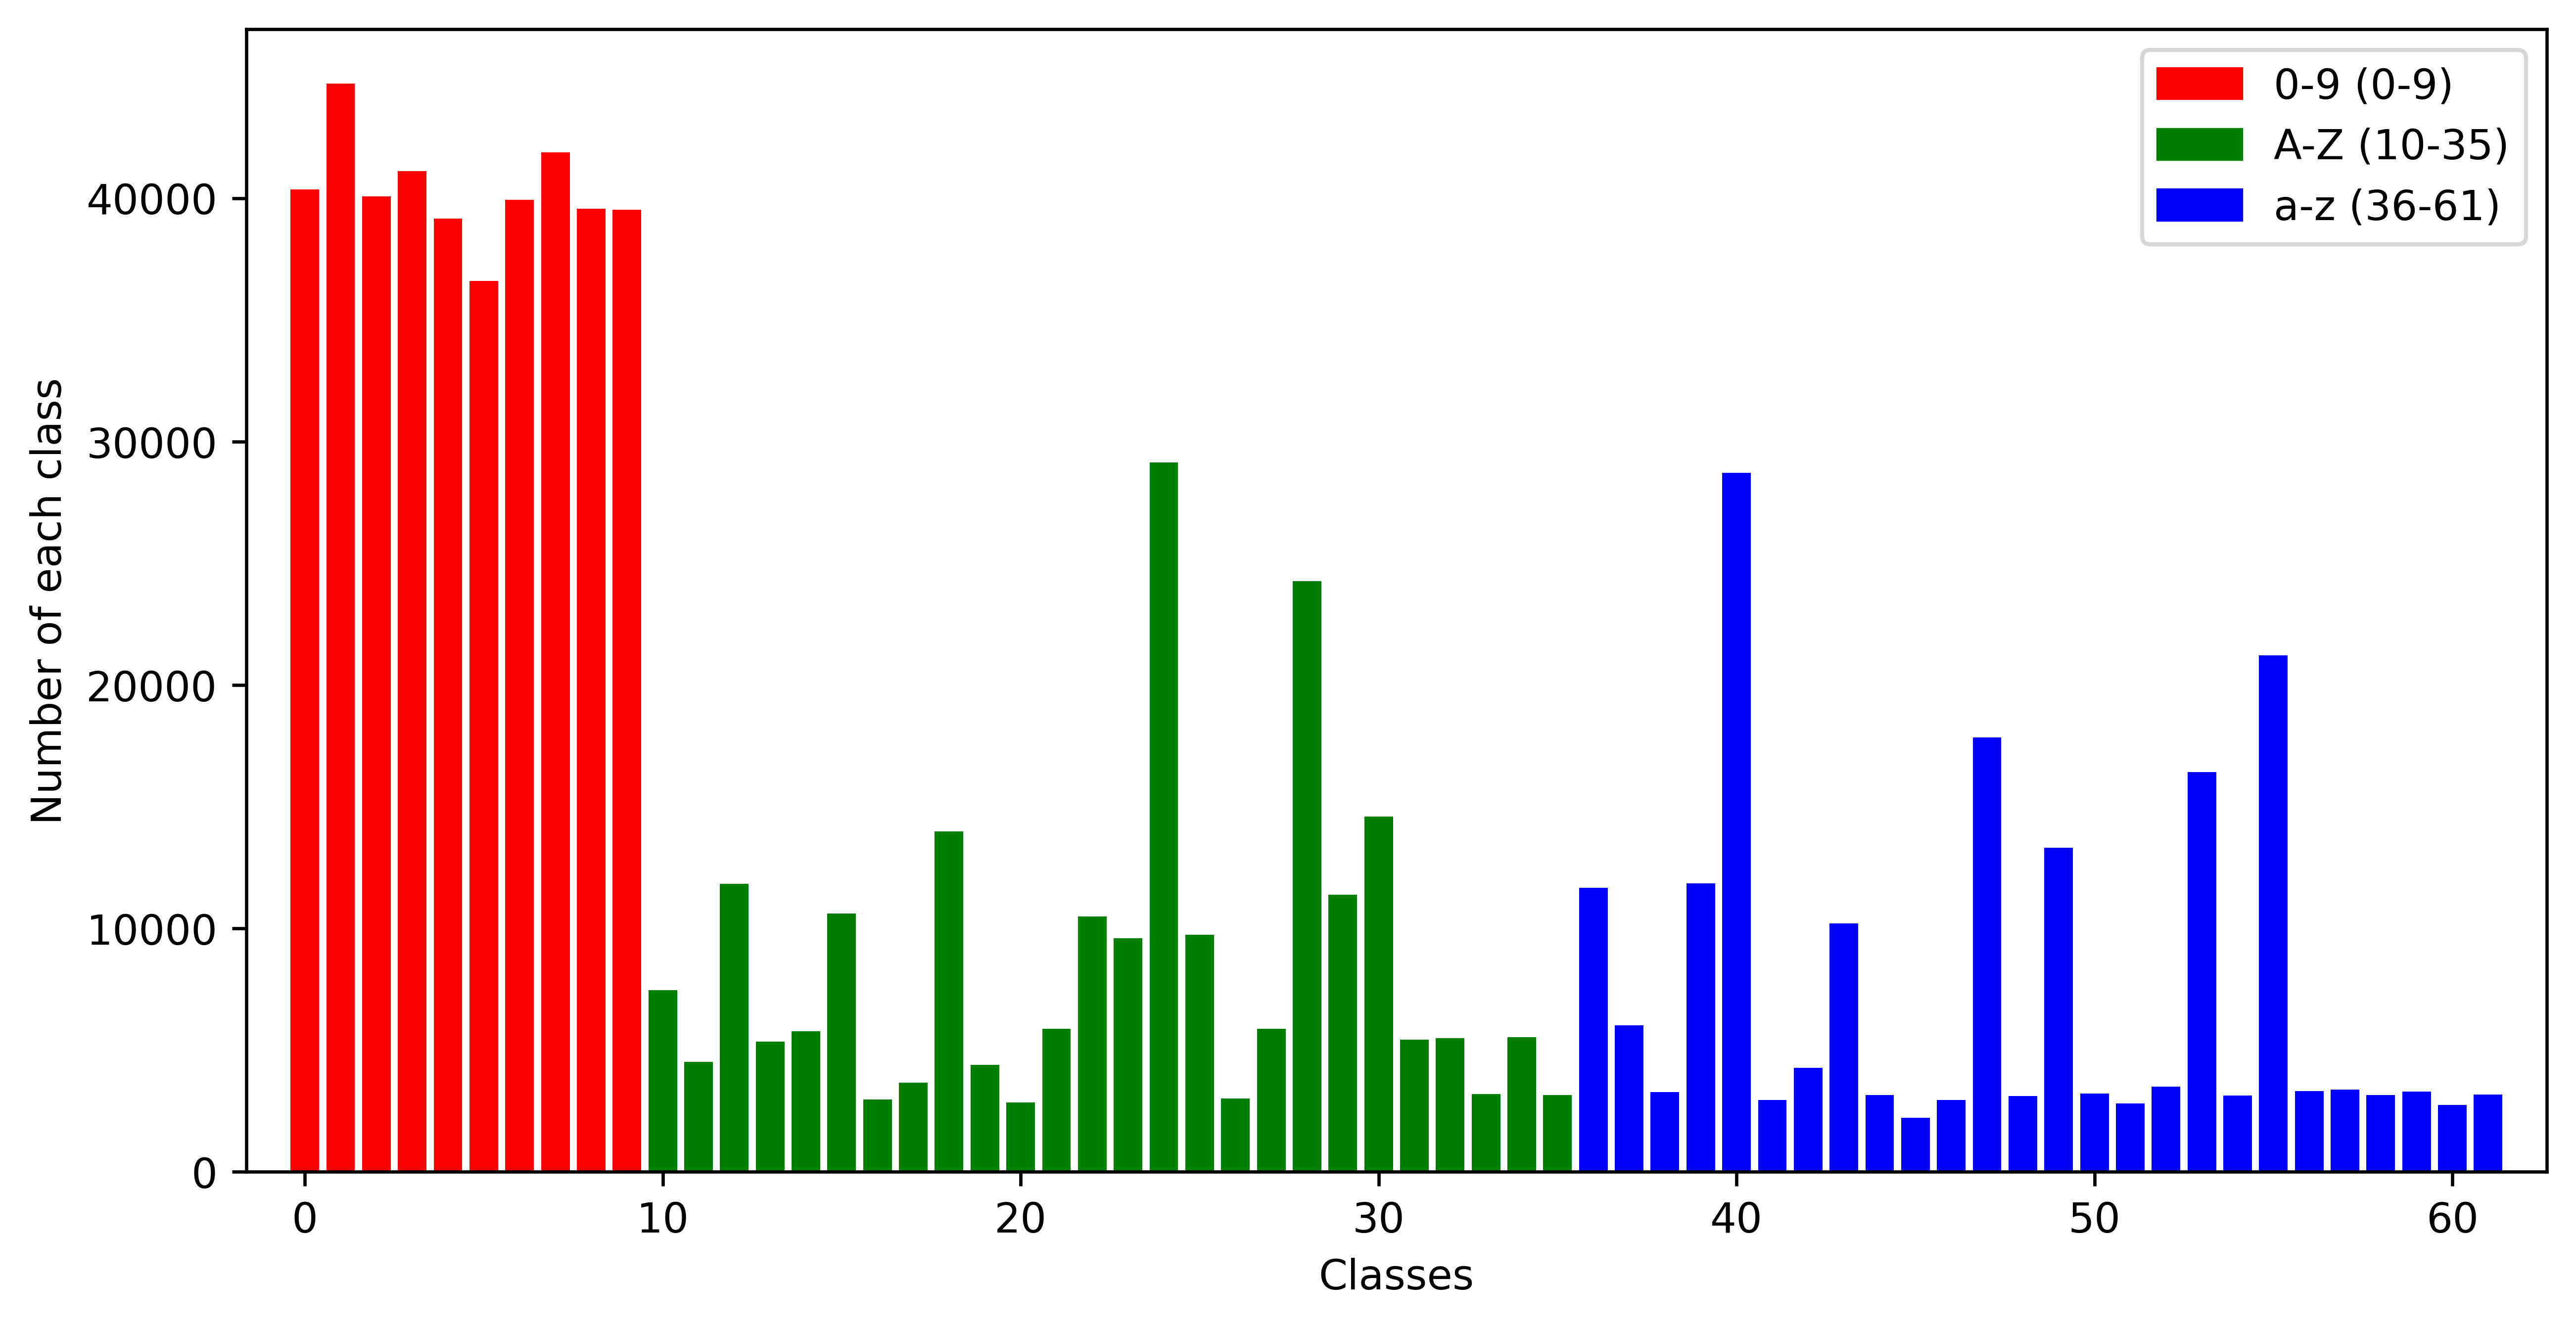
\includegraphics[scale=0.7]{images/chap5/count_all_classes.png}%
	\caption{%
		تعداد داده‌های هر کلاس و نحوه نام‌گذاری در مجموعه داده
		\lr{FEMNIST}.
	}
	\label{count_all_classes}
	\centering
\end{figure}

همان‌طور که در شکل
\ref{count_all_classes}
مشاهده می‌شود، تعداد کلاس‌های 0 تا 9 که به ارقام 0 تا 9 اشاره دارند، به‌طور قابل‌توجهی بیشتر از سایر کلاس‌هاست و هر کدام حدود 40٬000 نمونه دارند. در بین کلاس‌های 10 تا 35 که مربوط به حروف بزرگ انگلیسی هستند، کلاس‌های \lr{S} و \lr{O} بیشترین تعداد نمونه را دارند. به نظر می‌رسد این سبک از جمع‌آوری داده به دلیل جلوگیری از اشتباه گرفتن کلاس \lr{O} با عدد صفر و کلاس \lr{S} با معادل حرف کوچک آن در کلاس‌های 36 تا 61 بوده باشد.


مجموعه داده
\lr{FEMNIST}
به‌صورت پیش‌فرض شامل 3597 کاربر است که داده‌ها میان این کاربران توزیع شده‌اند. این توزیع، نه از لحاظ تعداد تصاویر بین کاربران و نه از لحاظ پوشش‌دهی کلاس‌ها در هر کاربر، یکسان نیست. با این حال، تعداد کاربران و نحوه توزیع داده‌ها میان آن‌ها را می‌توان به دلخواه تغییر داد.



اکنون رویکردهای پایه در مجموعه داده
\lr{FEMNIST}
بررسی خواهند شد. در رویکرد اول، داده‌ها بدون توجه به کاربران اصلی و تنها بر اساس کلاس‌های آن‌ها تفکیک می‌شوند. به این صورت که تمام داده‌های مربوط به هر کلاس جمع‌آوری شده و طبق یک توزیع مشخص بین تعدادی کاربر تقسیم می‌شوند. این روش به عنوان رویکرد کلاس‌بندی یا
\lr{FEMNISTclass}
شناخته می‌شود.

در رویکرد دوم، ساختار اصلی مجموعه داده تغییر نمی‌کند و تعداد کاربران همان تعداد پیش‌فرض باقی می‌ماند. همچنین داده‌ها دقیقا به همان شیوه‌ای که به هر کاربر اختصاص داده شده‌اند، حفظ می‌شوند. این روش به نام رویکرد نویسندگان یا
\lr{FEMNISTwriter}
نام‌گذاری شده است. در ادامه نتایج مربوط به هر کدام از این رویکرد‌ها به‌صورت مجزا بررسی خواهد شد.






\subsubsection{
	مقایسه نتایج در رویکرد کلاس‌بندی
	\lr{\texttt{\fontspec{Times New Roman} (FEMNISTclass)}}
}

نتایج مقایسه روش
\lr{SimFedSwap}
با دیگر روش‌های مرجع در شکل
\ref{result_FEMNISTclass}
نمایش داده شده‌اند که این آزمایش بر روی مجموعه داده
\lr{FEMNISTclass}
انجام شده است. پارامترهای مورد استفاده در این آزمایش نیز در جدول
\ref{tabel_parameter_FEMNISTclass}
ذکر شده‌اند.


\begin{figure}[t]
	\centering
	\subfigure[
	دید کلی از نتیجه
	\qquad\hspace{3mm}]{
		\label{result_FEMNISTclass_base}
		\includegraphics*[width=.48\textwidth]{images/chap5/result/FEMNISTclass/acc_base.png}
	}
	\hspace{0.8mm}
	\subfigure[
	بزرگ‌نمایی شده بخش اصلی					
	\qquad\hspace{5mm}]{
		\label{result_FEMNISTclass_zoom}
		\includegraphics*[width=.48\textwidth]{images/chap5/result/FEMNISTclass/acc_zoom.png}
	}
	\caption{
		مقایسه منحنی‌های دقت در مجموعه داده
		\lr{FEMNISTclass}.
	}
	\label{result_FEMNISTclass}
\end{figure}


%\addtolength{\tabcolsep}{-0.5mm}
\begin{table}[t]
	\centering
	\caption{
		پارامترهای اجرا در مجموعه داده
		\lr{FEMNISTclass}
	}
	\label{tabel_parameter_FEMNISTclass}
	%	\scalebox{0.985}{
		\begin{tabular}{ccccccccccccc}
			\hline
			\specialcell{مجموعه\\داده} &
			\specialcell{شبکه\\عصبی} &
			\specialcell{نحوه\\جابه‌جایی} &
			\specialcell{توزیع\\داده} &
			$K$ &
			$B$ &
			$C$ &
			$SP$ &
			$\eta$ &
			$E$ &
			$h_1$ &
			$h_2$
			\\
			\hline
			\lr{FEMNISTclass} &
			\lr{Conv} &
			\lr{MSS} &
			یکنواخت &
			\lr{200} &
			\lr{1024} &
			\lr{1.0} &
			\lr{1.0} &
			\lr{0.001} &
			\lr{2} &
			\lr{5} &
			\lr{3}
			\\
		\end{tabular}
		%	}
\end{table}



از شکل
\ref{result_FEMNISTclass}
مشخص است که روش‌های مبتنی‌بر جابه‌جایی در مقایسه با
\lr{FedAvg}
عملکرد متفاوتی نشان می‌دهند، اما همچنان تفاوت‌های عملکردی بین آن‌ها محدود و نزدیک به هم است.
نکته قابل توجه این است که بسیاری از تغییرات در نمودارها به لحظات جابه‌جایی یا میانگین‌گیری مربوط می‌شوند.
برای جزئیات بیشتر و بررسی دقیق‌تر، می‌توان به منحنی‌های خطا که در شکل
\ref{app_result_FEMNISTclass}
پیوست آمده‌اند، مراجعه کرد.




\subsubsection{
	مقایسه نتایج در رویکرد نویسندگان
	\lr{\texttt{\fontspec{Times New Roman} (FEMNISTwriter)}}
}
نتایج مربوط به مقایسه روش
\lr{SimFedSwap}
با سایر روش‌های مرجع در شکل
\ref{result_FEMNISTwriter_one}
قابل مشاهده است. این آزمایش بر روی مجموعه داده
\lr{FEMNISTwriter}
اجرا شده و پارامترهای به‌کاررفته در آن نیز در جدول
\ref{tabel_parameter_FEMNISTwriter}
ذکر شده‌اند.


\begin{figure}[t]
	\centering
	\subfigure[
	دید کلی از نتیجه
	\qquad\hspace{3mm}]{
		\label{result_FEMNISTwriter_one_base}
		\includegraphics*[width=.48\textwidth]{images/chap5/result/FEMNISTwriter/acc_base_one.png}
	}
	\hspace{0.8mm}
	\subfigure[
	بزرگ‌نمایی شده بخش اصلی					
	\qquad\hspace{5mm}]{
		\label{result_FEMNISTwriter_one_zoom}
		\includegraphics*[width=.48\textwidth]{images/chap5/result/FEMNISTwriter/acc_zoom_one.png}
	}
	\caption{
		مقایسه منحنی‌های دقت در یک اجرا بر روی مجموعه داده
		\lr{FEMNISTwriter}.
	}
	\label{result_FEMNISTwriter_one}
\end{figure}


%\addtolength{\tabcolsep}{-0.5mm}
\begin{table}[t]
	\centering
	\caption{
		پارامترهای اجرا در مجموعه داده
		\lr{FEMNISTwriter}
	}
	\label{tabel_parameter_FEMNISTwriter}
	%	\scalebox{0.985}{
		\begin{tabular}{ccccccccccccc}
			\hline
			\specialcell{مجموعه\\داده} &
			\specialcell{شبکه\\عصبی} &
			\specialcell{نحوه\\جابه‌جایی} &
			\specialcell{توزیع\\داده} &
			$K$ &
			$B$ &
			$C$ &
			$SP$ &
			$\eta$ &
			$E$ &
			$h_1$ &
			$h_2$
			\\
			\hline
			\lr{FEMNISTwriter} &
			\lr{Conv} &
			\lr{MSS} &
			یکنواخت &
			\lr{3597} &
			\lr{64} &
			\lr{0.15} &
			\lr{1.0} &
			\lr{0.001} &
			\lr{1} &
			\lr{5} &
			\lr{3}
			\\
		\end{tabular}
		%	}
\end{table}


در شکل
\ref{result_FEMNISTwriter_one}
مشاهده می‌شود که روش‌های مبتنی‌بر جابه‌جایی نتایجی متفاوت از روش
\lr{FedAvg}
ارائه داده‌اند. اما نکته مهم، برتری قابل توجه روش‌های مبتنی‌بر شباهت نسبت به
\lr{FedSwap}
است. این اولین آزمایشی است که در آن روش‌های شباهت محور توانسته‌اند عملکرد بهتری را به‌طور معناداری ارائه کنند. برای اطلاعات بیشتر و تحلیل دقیق‌تر، می‌توان به منحنی‌های خطا در شکل
\ref{app_result_FEMNISTwriter_one}
پیوست، مراجعه کرد.



با بهبود نتایج، این پرسش پیش می‌آید که آیا این برتری در شرایط استفاده از چندین
\lr{Seed}
متفاوت، همچنان پابرجا خواهد بود. برای پاسخ به این سوال، آزمایش قبلی با پنج
\lr{Seed}
مختلف تکرار شده و میانگین نتایج در شکل
\ref{result_FEMNISTwriter_seed}
نمایش داده شده‌اند. نکته قابل توجه این است که اختلاف روش مبتنی‌بر شباهت با روش
\lr{FedSwap}%
، دیگر به وضوح قبلی دیده نمی‌شود و تنها، بهبودی حدود یک درصد در میانگین پنج اجرا مشاهده می‌شود.
\begin{figure}[t]
	\centering
	\subfigure[
	دید کلی از نتیجه
	\qquad\hspace{3mm}]{
		\label{result_FEMNISTwriter_seed_base}
		\includegraphics*[width=.48\textwidth]{images/chap5/result/FEMNISTwriter/acc_base_seed.png}
	}
	\hspace{0.8mm}
	\subfigure[
	بزرگ‌نمایی شده بخش اصلی					
	\qquad\hspace{5mm}]{
		\label{result_FEMNISTwriter_seed_zoom}
		\includegraphics*[width=.48\textwidth]{images/chap5/result/FEMNISTwriter/acc_zoom_seed.png}
	}
	\caption{
		مقایسه منحنی‌های دقت در میانگین پنج اجرا بر روی مجموعه داده
		\lr{FEMNISTwriter}.
	}
	\label{result_FEMNISTwriter_seed}
\end{figure}
همچنین باید به این نکته توجه شود که تغییر
\lr{Seed}
در نمودارهای پیشین، تفاوت چشم‌گیری در خروجی ایجاد نمی‌کردند.
برای بررسی جزئیات بیشتر، منحنی‌های خطا در شکل
\ref{app_result_FEMNISTwriter_seed}
پیوست ارائه شده‌اند.


بنابراین می‌توان نتیجه گرفت که با افزایش تعداد کاربران و داده‌های مربوط به آن‌ها، روش‌های مبتنی بر شباهت، هرچند به میزان کم، می‌توانند عملکرد بهتری نشان دهند.
باید به این نکته توجه داشت که دقت کلی که در این مجموعه داده به 50 درصد رسید، وابسته به طراحی شبکه عصبی است. با بهینه‌سازی این شبکه، می‌توان به دقت بالاتری دست یافت. با این حال، این بهینه‌سازی تأثیری بر مقایسه بین روش‌ها نخواهد داشت، زیرا همه روش‌ها به‌طور همزمان به دقت بهتری دست خواهند یافت.


